\chapter{Acoustic emissions}

Modeling the acoustic emissions is a core feature of APECSS. To this end, APECSS offers different models for the acoustic emissions, assuming an incompressible liquid, a weakly-compressible liquid or a fully-compressible liquid. To account for a finite propagation speed, the information associated with an emitted acoustic wave is propagated along the radial coordinate axis using a Lagrangian wave tracking approach. Unless specifically told to do so, APECSS does not compute any acoustic emissions. 

\vspace{0.8em}

\noindent
\begin{tabular}{p{0.1\textwidth} p{0.32\textwidth} p{0.5\textwidth}}
    \textbf{Section} &\textbf{Command} & \textbf{Description} 
\vspace{1mm} \\ \hline
{\tt BUBBLE} & {\tt Emissions Incompressible} & Computes the acoustic emissions under the common incompressible assumption.\\ 
& {\tt Emissions FTI} & Computes the acoustic emissions under the assumption of an incompressible fluid but propagating the emissions with the speed of sound.\\ 
& {\tt Emissions QA} & Computes the acoustic emissions using the quasi-acoustic model of \citet{Gilmore1952}.\\ 
& {\tt Emissions EKB} & Computes the acoustic emissions using the explicit Kirkwood-Bethe model.\\ 
& {\tt Emissions GFC} & Computes the acoustic emissions using the fully-compressible model of \citet{Gilmore1952}.\\ 
& {\tt Emissions HPE} & Computes the acoustic emissions using the model of \citet{Hickling1963} and \citet{Ebeling1978}.\\ 
& {\tt EmissionIntegration Euler} & Integrates the radial position and, if applicable, the velocity using an Euler scheme.\\
& {\tt EmissionIntegration RK4} & Integrates the radial position and, if applicable, the velocity using a conventional fourth-order Runge-Kutta scheme. This is the default.\\
& {\tt KBIterTolerance <float>} & Tolerance $\eta$ for the evaluation of the pressure using a model based on the Kirkwood-Bethe hypothesis in conjunction with the NASG EoS.\\
 \hline
\end{tabular} \vspace{1em}

\section{Lagrangian wave tracking}

APECSS tracks acoustic emissions using a Lagrangian wave tracking approach, illustrated in Figure \ref{fig:lagrangiantracking}, in which so-called \textit{emission nodes} are propagated in the radial direction with propagation speed $\mathcal{C}$. Each emission node, represented in APECSS as a structure {\tt struct APECSS\_EmissionNode} and part of a linked list of these structures, holds the current radial coordinate $r(t)$, the flow velocity $u(r,t)$, the pressure $p(r,t$) and, if applicable, the enthalpy $h(r,t)$, as well as the invariants $f(\tau)$ and $g(\tau)$ computed based on the solution of the RP model. The radial position of an emission node at time $t$ is given as
\begin{equation}
    r(t) = R(\tau) + \int_\tau^t \mathcal{C}(r,t) \, \mathrm{d}t, 
    \label{eq:r_t}
\end{equation}
In general, the propagation speed is defined by $\mathcal{C}=c+u$, but the actual value used depends on the chosen model.

\begin{figure}
    \begin{center}
    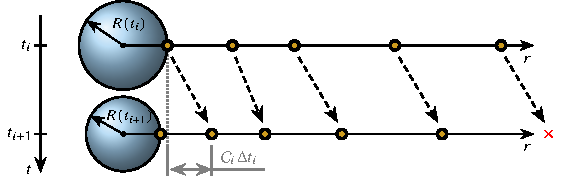
\includegraphics[width=0.7\linewidth]{LagrangianWaveTracking.pdf}
    \caption{Illustration of the Lagrangian transport of the emission nodes, updated at each discrete time instance $t_i$. Nodes that pass a predefined maximum radial coordinate are discarded.}
    \label{fig:lagrangiantracking}
    \end{center}
\end{figure}

\section{Incompressible assumption}

Assuming an incompressible liquid ($c_{\ell,\mathrm{ref}} \rightarrow  \infty$) with density $\rho_{\ell,\mathrm{ref}}$, the velocity $u(r,t)$ and pressure $p(r,t)$ at a given radial position $r(t)$ are defined as \citep{Neppiras1980}
\begin{equation}
    u(r,t) = \frac{R(t)^2 \dot{R}(t)}{r^2}  \label{eq:u_rt_incomp} 
\end{equation}
and 
\begin{equation}
    p(r,t) = p_\infty(t) + \rho_{\ell,\mathrm{ref}} \left[\frac{R(t)^2 \, \ddot{R}(t) + 2 \, R(t) \, \dot{R}(t)^2}{r} - \frac{R(t)^4 \, \dot{R}(t)^2}{2 \, r^4} \right], \label{eq:p_rt_incomp}
\end{equation}
respectively. The assumption of an incompressible fluid is consistent with the Rayleigh-Plesset models in Eqs.~\eqref{eq:standardRP} and \eqref{eq:modRP}. Note that, because $\mathcal{C} \rightarrow \infty$, these simple incompressible acoustic emissions do not use the Lagrangian wave tracking and no emission nodes are defined and processed, since pressure and velocity are defined instantaneously for all $r$.

Alternatively, APECSS also supports the assumption that the liquid is incompressible but the information associated with the acoustic emissions still propagates with finite speed $\mathcal{C} = c_{\ell,\mathrm{ref}}$ using the Lagrangian wave tracking approach. 
The radial location is then given as
\begin{equation}
    r(t) \approx R(\tau) + c_{\ell,\mathrm{ref}} \sum_{i=1}^N \Delta t_{i-1}. \label{eq:r_t_fti}
\end{equation}
This approach, referred to in APECSS as {\tt FTI} or \text{finite-time incompressible}, accurately recovers the time delay between emitting information at the bubble wall and this information arriving in a certain location.

\section{Quasi-acoustic model}
\label{sec:emissionsqa}

Assuming the liquid is compressible but accurately described by a constant density $\rho_{\ell,\mathrm{ref}}$ and constant speed of sound $c_{\ell,\mathrm{ref}}$, with $u \ll c_{\ell,\mathrm{ref}}$ and $\mathcal{C} = c_{\ell,\mathrm{ref}}$, \citet{Trilling1952} and \citet{Gilmore1952} derived the {\it quasi-acoustic model} for the acoustic emissions. With the quasi-acoustic model, the velocity, pressure and radial position follow as
\begin{align}
    u(r,t) &= \frac{f(\tau)}{r(t)^2} + \frac{g(\tau)}{r(t) \, c_{\ell,\mathrm{ref}}}  \label{eq:u_rt_qa} \\
  p(r,t) &=  p_\infty(t) + \rho_{\ell,\mathrm{ref}} \left[ \frac{g(\tau)}{r(t)} - \frac{u(r,t)^2}{2} \right] \label{eq:p_rt_qa} \\
  r(t) &\approx R(\tau) + c_{\ell,\mathrm{ref}} \sum_{i=1}^N \Delta t_{i-1}, \label{eq:r_t_qa}
\end{align}
where $f(\tau)$ and $g(\tau)$ are invariants defined based on the result of the employed RP model as
\begin{align}
    f(\tau) &= R(\tau)^2 \dot{R}(\tau) - \frac{R(\tau) g(\tau)}{c_{\ell,\mathrm{ref}}}\\
    g(\tau) &= R(\tau) \left[\frac{p_\mathrm{L}(\tau)-p_\infty}{\rho_{\ell,\mathrm{ref}}} + \frac{\dot{R}(\tau)^2}{2} \right],
\end{align}
and $\tau$ is the time at which the acoustic information is emitted at the bubble wall. For $t=\tau$ with $r=R(\tau)$, Eq.~(\ref{eq:u_rt_qa}) reduces to $u(R,\tau)=\dot{R}(\tau)$ and Eq.~(\ref{eq:p_rt_qa}) reduces to $p(R,\tau)=p_\mathrm{L}(\tau)$, thus satisfying the boundary conditions at the bubble wall. 

The quasi-acoustic model is consistent in its modelling assumptions with the Keller-Miksis model, Eq.~\eqref{eq:keller}. The applicability of the quasi-acoustic model is limited to small Mach numbers, $(\dot{R}/c_0)^2 \ll 1$, as it incorporates a finite propagation speed of the acoustic emissions and the nonlinear pressure contributions resulting from the flow, but since all parts of the wave propagate with speed $c_0$, the quasi-acoustic model can neither describe the nonlinear distortion of acoustic waves nor the formation of shock fronts. 

\section{Emissions based on the Kirkwood-Bethe hypothesis}
\label{sec:emissionskb}

Under the Kirkwood-Bethe hypothesis \citep{Kirkwood1942,Cole1948}, the propagation speed along the outgoing characteristic is given as $\mathcal{C}(r,t) = c(r,t) + u(r,t)$. The ODE describing 
the radial position is, thus, defined as 
\begin{equation}
    \frac{\mathrm{d}r(t)}{\mathrm{d}t} = c(r,t) + u(r,t). \label{eq:drdt}
\end{equation}
This ODE is numerically integrated using either an Euler scheme or a fourth-order Runge-Kutta (RK4) scheme, with initial condition $r(\tau) = R(\tau)$, where  $\tau$ is the time at which the acoustic information is emitted at the bubble wall. The time-step $\Delta t$ is taken to be the same as used for the integration of the model describing the bubble dynamics (see Section \ref{chap:bubble}).

Three models to compute the velocity $u(r,t)$ at a given emission node are available in APECSS: (i) an explicit expression for $u(r,t)$, (ii) integrating the spatial derivative of the velocity, $\mathrm{d}u(r,t)/\mathrm{d}r$, along the outgoing characteristic, as proposed by \citet{Gilmore1952}, and (iii) integrating the temporal derivative of the velocity, $\mathrm{d}u(r,t)/\mathrm{d}t$, along the outgoing characteristic, as proposed by \citet{Hickling1963}.
The assumptions used to derive these models for the acoustic emissions are consistent with the Gilmore model, Eq.~\eqref{eq:gilmore}.

Following a similar derivation as for the quasi-acoustic model discussed in Section \ref{sec:emissionsqa}, but assuming a fully-compressible liquid described by a suitable equation of state, the velocity is given by the {\it explicit Kirkwood-Bethe (EKB)} model as
\begin{equation}
    u(r,t) = \frac{f(\tau)}{r(t)^2} + \frac{g(\tau)}{r(t) \, \mathcal{C}(r,t)} . \label{eq:u_rt},
\end{equation}
For $t=\tau$ with $r=R(\tau)$, this expression reduces to $u(R,\tau)=\dot{R}(\tau)$, thus satisfying the boundary conditions at the bubble wall.
\citet{Gilmore1952} proposed instead to solve for the spatial derivative of the velocity along the outgoing characteristic, in APECSS referred to as {\it Gilmore's fully compressible (GFC)} model, with the velocity defined by 
\begin{equation}
    \frac{\mathrm{d}u(r,t)}{\mathrm{d}r} = - \frac{2 u(r,t)}{r(t)} \left[1+\frac{u(r,t)^2}{c(r,t)^2-u(r,t)^2} \right] + \frac{g(\tau)}{r(t)^2 [c(r,t)-u(r,t)]} \label{eq:dudr_rt}.
\end{equation}
Alternatively, \citet{Hickling1963} proposed to integrate the velocity with respect to time, in APECSS referred to as {\it Hickling-Plesset-Ebeling (HPE)} model, with the temporal derivative of the velocity along the outgoing characteristic given as
\begin{equation}
    \frac{\mathrm{d}u(r,t)}{\mathrm{d}t} =  - \frac{2 c(r,t)^2 u(r,t)}{r(t) \, [c(r,t)-u(r,t)]} + \frac{g(\tau)}{r(t)^2} \, \frac{c(r,t)+u(r,t)}{c(r,t)-u(r,t)}. \label{eq:dudt_rt}
\end{equation}
If either Eq.~\eqref{eq:dudr_rt} or Eq.~\eqref{eq:dudt_rt} is chosen to determine the velocity, this differential equation for velocity is integrated together with the equation for ${\mathrm{d}r(t)/\mathrm{d}t}$, Eq.~\eqref{eq:drdt}, using the initial condition $u(R,\tau) = \dot{R}(\tau)$. Note that with $\mathrm{d}r(t)/\mathrm{t}$ defined by Eq.~\eqref{eq:drdt} and $g(\tau)$ given by Eq.~\eqref{eq:g_R}, Eqs.~\eqref{eq:dudr_rt} and \eqref{eq:dudt_rt} are interchangeable by the relation ${\mathrm{d}u/\mathrm{d}t} = ({\mathrm{d}u/\mathrm{d}r}) \, ({\mathrm{d}r/\mathrm{d}t})$. 

Regardless of the choice of velocity model, the invariants $f(\tau)$ and $g(\tau)$ are defined as
\begin{align}
    f(\tau) &= R(\tau)^2 \dot{R}(\tau) - \frac{R(\tau) \, g(\tau)}{c_\mathrm{L}(\tau) + \dot{R}(\tau)}   \label{eq:f_R} \\  
    g(\tau) &= R(\tau) \left[h_\mathrm{L}(\tau) - h_\infty(\tau) + \frac{\dot{R}(\tau)^2}{2} \right]
    \label{eq:g_R} ,
\end{align}
For a given radial position $r(t)$ and flow velocity $u(r,t)$, irrespective of which model is used to compute the velocity, the enthalpy is then readily evaluated as
\begin{equation}
    h(r,t) = h_\infty(t) + \frac{g(\tau)}{r(t)} - \frac{u(r,t)^2}{2}, \label{eq:h_rt}
\end{equation}
where $h_\infty$ is spatially invariant and only depends on time.
For $t=\tau$ with $r=R(\tau)$, this expression for enthalpy reduces to $h(R,\tau)=h_\mathrm{L}(\tau)$, satisfying the boundary conditions at the bubble wall. 

Using the Tait EoS, the pressure can be readily computed from the enthalpy defined in Eq.~(\ref{eq:h_rt}) by inserting Eq.~(\ref{eq:rho_Tait}) into Eq.~(\ref{eq:h_Tait}) and rearranging to yield
\begin{equation}
    p(r,t) = \left[ \frac{(\Gamma-1) \, \rho_0}{\Gamma \, (p_0+B)^{1/\Gamma}} \, h(r,t) \right]^{\frac{1}{1-1/\Gamma}} - B. \label{eq:p_rt}
\end{equation}
Solving Eq.~(\ref{eq:p_rt}) is straightforward because the enthalpy $h(r,t)$ is the only variable, all other quantities are predefined fluid properties. Using the NASG EoS, pressure $p(r,t)$ follows by rearranging Eq.~(\ref{eq:h_NASG}) as
\begin{eqnarray}
p(r,t) = \frac{\left[\Gamma-1\right] \rho(r,t) \, h(r,t) - \left[1 - b \, \rho(r,t) \right] \Gamma B}{\Gamma - b \, \rho(r,t)}.  \label{eq:p_rt_NASG}
\end{eqnarray}
Since the pressure $p(r,t)$ and the density $\rho(r,t)$ depend explicitly on each other in this formulation, Eq.~(\ref{eq:p_rt_NASG}) has to be solved iteratively. As a convergence criterion for the iterative approximation we use $|p_j(r,t) - p_{j-1}(r,t)| < \eta \, |p_j(r,t)|$, where $j$ denotes the iteration counter and $\eta$ is a predefined tolerance (see option {\tt KBIterTolerance}). Preliminary tests identified a tolerance of $\eta = 10^{-4}$ to be sufficiently small.


Emission nodes with a higher pressure propagate faster than nodes with a lower pressure, which in turn leads to progressive steepening of the acoustic wave. As a result, an emission node may overtake the forerunning emission node, yielding an unphysical multivalued solution. In reality, such a multivalued solution is avoided by the formation of a shock front \citep{Fay1931}. While treating such multivalued solutions is often done in a post-processing step, APECSS deals with multivalued solutions on-the-fly. \citet{Rudnick1952} postulated that the rate of attenuation of a stable shock front is independent of the dissipation process leading to the stable shock front. Exploiting Rudnick's argument, an emission node that overtakes its forerunning neighbor is simply discarded in APECSS, see Fig.~\ref{fig:lagrangiantrackingshock}, thus maintaining a physically plausible solution.

\begin{figure}
    \begin{center}
    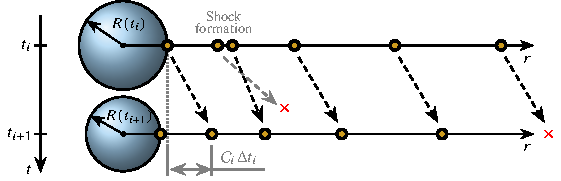
\includegraphics[width=0.7\linewidth]{LagrangianWaveTracking_withShock.pdf}
    \caption{Illustration of the Lagrangian transport of the emission nodes, updated at each discrete time instance $t_i$. Nodes that either overtake the forerunning node, which represents the formation of a shock front, or that pass a predefined maximum radial coordinate are discarded.}
    \label{fig:lagrangiantrackingshock}
    \end{center}
\end{figure}


\section{Results}

APECSS can write out different results based on the acoustic emissions. Note that APECSS does \uline{not} write any results to disk unless it is specifically ask to do so.

The acoustic emissions can be recorded as a function of time at one or multiple radial locations (cf.~{\tt EmissionsSpace}), or the emissions are written out with respect to their radial location at one or multiple time instances (cf.~{\tt EmissionsTime}) or emission nodes (cf.~{\tt EmissionsNode}), or for selected extrema in a specified period (cf.~{\tt EmissionsMinMax}). This calls can be used multiple times to defined, for instance, multiple radial locations or time instances.

\vspace{0.8em}

\noindent
\begin{tabular}{p{0.1\textwidth} p{0.36\textwidth} p{0.49\textwidth}}
    \textbf{Section} &\textbf{Command} & \textbf{Description} 
\vspace{1mm} \\ \hline
{\tt RESULTS} & {\tt OutputPath <string>} & Path to the folder where all the results should be written in to (default: {\tt ./}).\\
& {\tt OutputDigits <int>} & Results are written out with as many digits (default: 6).\\
& {\tt EmissionsSpace <float>} & Defines a radial location at which the emissions in the liquid are written out as a function of time. If/while the location is in the gas phase, $0$ is recorded.\\ 
& {\tt OutputFreqEmissionsSpace <int>} & Results of the emissions at a specific radial location are stored every so many time steps (default: 1).\\ 
& {\tt EmissionsTime <float>} & Defines a time instance at which the emission in the liquid are written out as a function of the radial coordinate.\\ 
& {\tt EmissionsNode <int>} & Defines a node ID of which the emission in the liquid are written out as a function of the radial coordinate.\\ 
& {\tt EmissionsMinMax <int>} & Defines the period in which the emission in the liquid are written out as a function of the radial coordinate for the node representing $R_\mathrm{min}$, $\dot{R}_\mathrm{min}$ and $p_\mathrm{L,max}$.\\ 
 \hline
\end{tabular}

The first line of the results file(s) lists the variables that were written out and their order.